% =====================================================================
%  FoodGenome AI — project report
%  East Delta University
%
%  Build:  ./build.sh      (or: tectonic paper.tex)
%
%  Every figure is generated by figures.py from the evaluation artifacts.
%  No number in this document was transcribed by hand.
% =====================================================================

\documentclass[11pt,a4paper,twoside]{article}

% ---------------------------------------------------------------------
%  >>> CHECK THESE BEFORE SUBMITTING <<<
% ---------------------------------------------------------------------
\newcommand{\StudentName}{A K M Asifuzzaman}
\newcommand{\StudentID}{000000000}          % <-- replace with your real student ID
\newcommand{\CourseCode}{CSE 450 Python Project}
\newcommand{\Instructor}{Arshiana Shamir}
\newcommand{\SubmissionDate}{August 2026}
% ---------------------------------------------------------------------

\usepackage[T1]{fontenc}
\usepackage[utf8]{inputenc}
\usepackage{lmodern}
\usepackage{microtype}
\usepackage[a4paper,margin=1.05in]{geometry}
\usepackage{graphicx}
\usepackage{xcolor}
\usepackage{booktabs}
\usepackage{amsmath}
\usepackage{caption}
\usepackage{subcaption}
\usepackage{enumitem}
\usepackage{titlesec}
\usepackage{fancyhdr}
\usepackage[hidelinks]{hyperref}

\definecolor{edumaroon}{RGB}{128,20,40}
\definecolor{inkgrey}{RGB}{70,70,70}

\captionsetup{font=small,labelfont={bf,color=edumaroon},width=0.94\textwidth}
\titleformat{\section}{\large\bfseries\color{edumaroon}}{\thesection}{0.7em}{}
\titleformat{\subsection}{\normalsize\bfseries}{\thesubsection}{0.6em}{}
\setlist[itemize]{leftmargin=1.3em,itemsep=1pt,topsep=3pt}
\setlength{\parskip}{0.35em}

\pagestyle{fancy}
\fancyhf{}
\fancyhead[LE,RO]{\small\textcolor{inkgrey}{FoodGenome AI}}
\fancyhead[RE,LO]{\small\textcolor{inkgrey}{\StudentName}}
\fancyfoot[C]{\small\thepage}
\renewcommand{\headrulewidth}{0.4pt}

\newcommand{\num}[1]{\mbox{#1}}

\begin{document}

% ── Title ────────────────────────────────────────────────────────────
\begin{titlepage}
\centering
\vspace*{1.2cm}
{\Large\bfseries\color{edumaroon} FoodGenome AI\par}
\vspace{0.4cm}
{\large Calibrated Food Recognition with Conformal Guarantees\\and Grounded Nutritional Retrieval\par}
\vspace{1.4cm}
{\normalsize\itshape What five negative results taught us about\\when added complexity does not pay\par}
\vspace{2.2cm}
\begin{tabular}{rl}
\textbf{Author}      & \StudentName \\
\textbf{Student ID}  & \StudentID \\
\textbf{Course}      & \CourseCode \\
\textbf{Instructor}  & \Instructor \\
\textbf{Date}        & \SubmissionDate \\
\end{tabular}
\vfill
{\small Source, live demonstration and all evaluation artifacts:\\
\url{https://github.com/A-K-M-Asifuzzaman/Food} \quad\textbullet\quad
\url{https://food-red-omega.vercel.app}\par}
\vspace{0.8cm}
\end{titlepage}

% ── Abstract ─────────────────────────────────────────────────────────
\begin{abstract}
\noindent
We present FoodGenome~AI, an end-to-end system that classifies a photographed dish into one
of the 101 Food-101 categories, reports a calibrated confidence, returns a conformal
prediction set carrying a measured coverage guarantee, and answers natural-language
questions about the dish from a USDA-grounded knowledge base without stating any figure it
cannot cite.

An ensemble of two frozen vision backbones reaches \num{97.16\%} top-1 on the held-out test
split. Temperature scaling reduces expected calibration error \num{8.2}-fold, and
split-conformal prediction attains \num{99.56\%} empirical coverage at a mean set size of
\num{1.54}. A retrieval pipeline combining lexical and dense search answers \num{98.6\%} of a
76-case gold set correctly, refuses \num{100\%} of out-of-scope questions, and grounds every
numeric claim against a retrieved source.

The contribution we consider most useful is negative. Five hypotheses that a practitioner
would reasonably expect to hold did not: a trained fusion head lost to a parameter-free
average; a self-supervised third backbone predicted to decorrelate proved the most
correlated; attention-pooling maps localised the subject \emph{worse than chance}; a
conformal implementation whose calibration and deployment rules differed produced a
better-looking number from a void guarantee; and end-to-end fine-tuning improved the
ensemble by only \num{0.11} points, short of significance at $p=0.052$. Each was established
with an exact McNemar test or a measured baseline rather than by inspection.
\end{abstract}

\tableofcontents
\newpage

% ── 1 ────────────────────────────────────────────────────────────────
\section{Introduction}

Food recognition is an attractive application of computer vision because the output is
immediately useful: a diner who photographs a plate wants to know what is on it and what it
contains. It is also a domain where being confidently wrong carries real cost. A nutrition
figure presented without qualification will be acted on, and a classifier restricted to 101
categories will return one of them for a photograph of anything at all.

This project therefore treats \emph{knowing when not to answer} as a first-class requirement
alongside accuracy. Three mechanisms implement that: a calibrated confidence whose numeric
value corresponds to observed correctness, a conformal prediction set with a coverage
guarantee that holds without distributional assumptions about the model, and an abstention
rule that declines images the model cannot resolve. A fourth applies to the language side: a
grounding gate that withholds any generated answer containing a quantity absent from its
retrieved sources.

\subsection{Contributions}

\begin{itemize}
  \item An ensemble reaching \num{97.16\%} Food-101 top-1 on a test split untouched until
        final evaluation, with model selection performed on a fixed validation slice carved
        from the training set.
  \item A calibration and conformal-prediction pipeline delivering a measured \num{99.56\%}
        coverage guarantee at a mean set size of \num{1.54}, and an abstention rule that
        raises accuracy on accepted images to \num{97.94\%}.
  \item A retrieval-augmented question-answering system with a numeric grounding gate,
        evaluated on a gold set whose ground truth is derived rather than judged.
  \item Five negative results, each established by significance test or measured baseline,
        which together argue that added complexity in this setting frequently does not pay.
\end{itemize}

% ── 2 ────────────────────────────────────────────────────────────────
\section{Method}

\subsection{Data and the validation protocol}

Food-101 \cite{bossard2014} contains \num{101{,}000} images across 101 classes, distributed
as \num{75{,}750} training and \num{25{,}250} test images. It ships no validation split.
Reporting model-selection numbers on the test set is the most common way work of this kind
overstates itself, so a fixed \num{4\%} class-stratified slice (\num{3{,}030} images, seed
1337) is carved from the training set and shared by every stage. The test split is untouched
until final evaluation.

Because the fine-tuning stage ran on separate hardware, the validation mask is hashed and
the hash asserted before training is permitted to begin. A divergent slice would make the
two sets of results incomparable and would leak validation data into any ensemble of them.
Both label arrays were later confirmed byte-identical across machines.

\subsection{Frozen feature bank}

Three backbones --- SigLIP-SO400M \cite{zhai2023}, EVA-02-L \cite{fang2023} and DINOv2-L
\cite{oquab2023} --- were run once over the full corpus and their pooled embeddings cached, a
one-time cost of roughly twenty hours. Every subsequent experiment (head architecture,
calibration, conformal sets, abstention, ensembling) then completes in seconds rather than
hours. This is what made the ablation in Section~\ref{sec:ablation} affordable: it was rerun
dozens of times.

Lightweight MLP heads (\num{1.7}--\num{1.9}M parameters) are trained on the cached features
with mixup and label smoothing. Features are $L_2$-normalised before the head, which must be
replicated at inference.

\subsection{Reliability}

Let $p_\theta(y \mid x)$ denote the ensemble's output. A single scalar temperature $T$ is
fitted on the validation slice by minimising negative log-likelihood, giving calibrated
probabilities $\mathrm{softmax}(\log p_\theta / T)$. Temperature scaling is monotonic and so
cannot alter accuracy; it alters only what the reported number means.

For conformal prediction we use split-conformal with the LAC score $s(x,y) = 1 -
\hat{p}(y\mid x)$ \cite{sadinle2019}. Given miscoverage $\alpha$, the threshold $\hat{q}$ is
the $\lceil (n+1)(1-\alpha)\rceil / n$ empirical quantile of calibration scores, and the
prediction set is $\{y : \hat{p}(y \mid x) \ge 1-\hat{q}\}$. The finite-sample correction is
not cosmetic: at $n=3030$ omitting it under-covers.

\subsection{Retrieval and grounding}

The knowledge base holds all 101 classes with 32 USDA nutrients each. USDA SR Legacy
contains a direct record for 41; the remaining 60 are composed from weighted ingredient
records, and every surface states which of the two a figure is.

Retrieval fuses BM25 and a bi-encoder by Reciprocal Rank Fusion \cite{cormack2009} rather
than by weighted score sum: BM25 scores are unbounded while cosine similarity is bounded,
so any weighted combination requires a normalisation constant that is itself tuned. A
cross-encoder then reranks. Crucially, the query is rewritten to name the dish the vision
model has already identified --- real questions contain pronouns (``how much sodium is in
\emph{this}''), which no retriever can resolve against 101 near-identical documents.

Generation is constrained to the retrieved context, and every quantity in the output is
verified against that context before display, matched per unit so that milligrams cannot be
supported by the same digits in grams. An answer that fails is withheld and a deterministic
summary of the retrieved record served instead.

% ── 3 ────────────────────────────────────────────────────────────────
\section{Results}

\subsection{Single models and the ablation}
\label{sec:ablation}

\begin{table}[htbp]
\centering\small
\caption{Individual heads on the held-out test split. Frozen-feature performance tracks
pretraining data rather than architecture: SigLIP's caption supervision already encodes food
semantics.}
\begin{tabular}{lrrrr}
\toprule
\textbf{Head} & \textbf{Params} & \textbf{Val top-1} & \textbf{Test top-1} & \textbf{Test top-5} \\
\midrule
SigLIP-SO400M           & \num{1.93}M & \num{95.64} & \textbf{\num{96.83}} & \num{99.53} \\
EVA-02-L                & \num{1.73}M & \num{93.14} & \num{95.53} & \num{99.30} \\
DINOv2-L                & \num{1.73}M & \num{92.64} & \num{94.87} & \num{99.20} \\
Gated fusion head       & \num{3.97}M & --          & \num{96.97} & \num{99.48} \\
EVA-02-L fine-tuned     & \num{304}M  & \num{92.94} & \num{95.90} & \num{99.52} \\
\bottomrule
\end{tabular}
\end{table}

\begin{figure}[htbp]
\centering
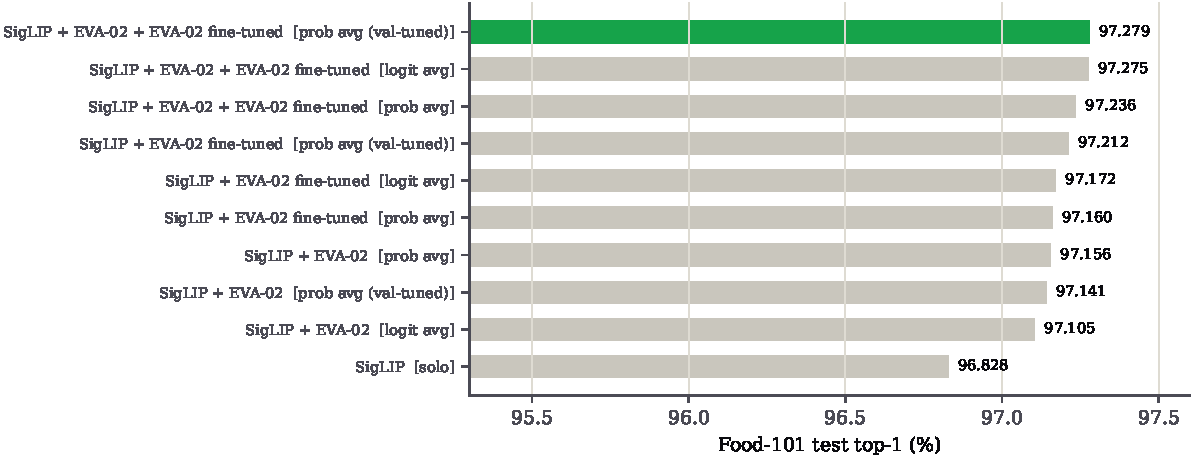
\includegraphics[width=0.98\textwidth]{figures/ablation.pdf}
\caption{Every combination evaluated. The best configuration is a weighted probability
average with no learned parameters.}
\label{fig:ablation}
\end{figure}

\paragraph{Negative result 1: a trained fusion head lost to arithmetic.}
A gated fusion head with \num{3.97}M parameters, trained for \num{21.9} minutes to weight
each backbone per input, reached \num{96.97\%}. A parameter-free \num{50}/\num{50} average of
the same two probes reached \num{97.16\%} in milliseconds. An exact McNemar test on paired
predictions puts the average ahead at $p = \num{0.005}$, while the fusion head does
\emph{not} significantly beat its own best single input ($p = \num{0.071}$). With two heavily
correlated members, the additional capacity purchases variance rather than signal.

\paragraph{Negative result 2: the third backbone earned no place.}
DINOv2-L is the only self-supervised member and was therefore predicted to make the most
independent errors. It makes the least: \num{66.3\%} of SigLIP's errors are shared with it,
against \num{65.2\%} with EVA-02. Adding it moved the three-way average to \num{97.09\%},
marginally below the pair, at $p = \num{0.312}$ --- not a significant loss, but no gain
either. A validation weight search independently drove its weight to \num{0.05}.

\subsection{Calibration and conformal prediction}

\begin{figure}[htbp]
\centering
\begin{subfigure}[b]{0.46\textwidth}
  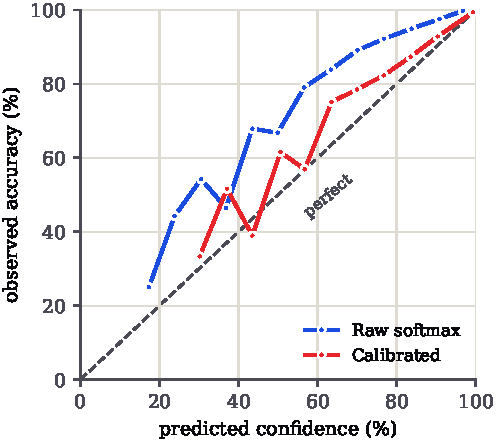
\includegraphics[width=\textwidth]{figures/reliability.pdf}
  \caption{Reliability diagram. The ensemble sat \emph{above} the diagonal --- systematically
  under-confident, the less common direction.}
  \label{fig:reliability}
\end{subfigure}\hfill
\begin{subfigure}[b]{0.46\textwidth}
  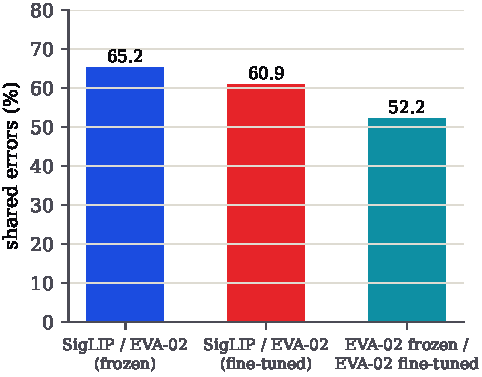
\includegraphics[width=\textwidth]{figures/decorrelation.pdf}
  \caption{Shared-error rate. Fine-tuning at 448\,px is what produced diversity; at 224\,px
  it produced none.}
  \label{fig:decorrelation}
\end{subfigure}
\caption{Reliability and diversity.}
\end{figure}

Temperature scaling fitted $T = \num{0.7621}$, reducing expected calibration error from
\num{0.0514} to \num{0.0062} --- a factor of \num{8.2}. Mean confidence moved from
\num{92.0\%} to \num{96.6\%} against \num{97.16\%} accuracy; the two now agree.

\begin{table}[htbp]
\centering\small
\caption{Conformal coverage against mean set size. Below the model's own top-1 accuracy the
guarantee is satisfied by the single best prediction and the ``set'' degenerates to one
class.}
\begin{tabular}{lrrrr}
\toprule
\textbf{Target} & \textbf{Method} & \textbf{Coverage} & \textbf{Mean size} & \textbf{Singletons} \\
\midrule
\num{90\%} & LAC       & \num{93.59} & \num{0.95} & \num{94.6\%} \\
\num{90\%} & APS       & \num{90.18} & \num{1.54} & \num{80.4\%} \\
\num{95\%} & APS       & \num{95.56} & \num{2.52} & \num{79.7\%} \\
\num{99\%} & LAC + top-1 & \textbf{\num{99.56}} & \textbf{\num{1.54}} & \num{75.9\%} \\
\bottomrule
\end{tabular}
\end{table}

\paragraph{Negative result 3: a mismatched conformal rule looked better.}
An initial implementation forced the top-1 class into the prediction set at test time while
scoring \emph{without} it during calibration. This silently rescued the \num{13\%} of images
whose top score exceeded the threshold, producing \num{99.1\%} empirical coverage against a
\num{90\%} target. The guarantee was void, and the reported number was \emph{better} for it
--- which is what makes this class of error dangerous. Conformal validity requires the
identical rule in calibration and deployment; after correction, APS attains \num{90.18\%}
against a \num{90\%} target.

\paragraph{Abstention.} Neither available signal suffices alone. A maximum-probability
threshold rejects noise but admitted a flat colour field at \num{0.43}, classified
``breakfast burrito''. Conformal set size caught that at eight candidates where correctly
classified dishes return one. Their disjunction abstains on \num{2.28\%} of real food and
raises accuracy on the remainder from \num{97.16\%} to \num{97.94\%}. This is an abstention
rule, not a trained out-of-distribution detector: it reports that the model is lost, which
correlates with but does not equal ``this is not food''.

\subsection{Explainability}

\begin{figure}[htbp]
\centering
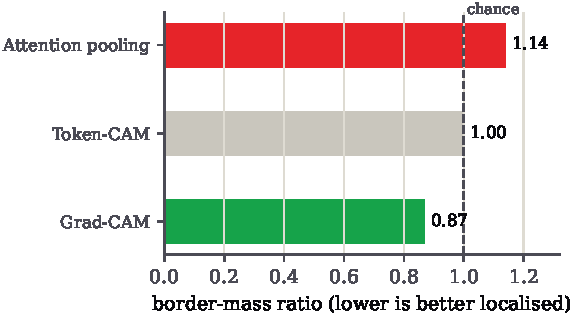
\includegraphics[width=0.62\textwidth]{figures/attribution.pdf}
\caption{Attribution localisation, measured as the share of attribution mass falling in the
outer ring of the frame (\num{60\%} of the area) over 24 test images. Food-101 subjects are
typically centred, so lower is better.}
\label{fig:attribution}
\end{figure}

\paragraph{Negative result 4: attention is not saliency.}
Reading the pooling head's own attention weights ought to be the most faithful account of
where the model looked --- those weights are literally the mixture forming the classified
vector. Measured against a border-mass baseline, it is \emph{worse than chance} at locating
the subject (\num{1.14}$\times$), while classic Grad-CAM \cite{selvaraju2017} reaches
\num{0.87}$\times$ and is also far more class-discriminative (map correlation $r=+0.07$
between two target classes, against $r=+0.38$ for token-level attribution). This reproduces
the documented tendency of vision transformers to place high attention on low-information
background patches \cite{darcet2024}.

Localisation is weak in absolute terms for all three methods, and the cause is
architectural: the classifier sees only a globally pooled vector, so spatial attribution
must be recovered through a step that discarded position.

\subsection{Fine-tuning}

\begin{figure}[htbp]
\centering
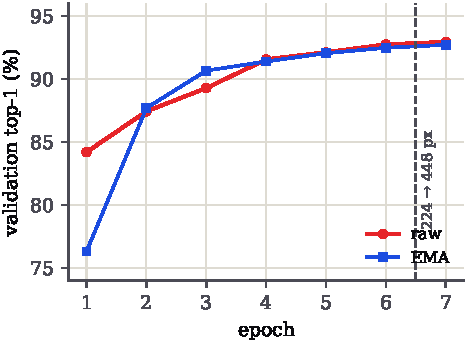
\includegraphics[width=0.55\textwidth]{figures/training.pdf}
\caption{Fine-tuning EVA-02-L: six epochs at 224\,px followed by one at 448\,px. The
resolution change contributes \num{0.2} points of validation accuracy.}
\label{fig:training}
\end{figure}

\paragraph{Negative result 5: fine-tuning decorrelated but did not significantly win.}
End-to-end fine-tuning reached \num{95.90\%} alone --- below the frozen ensemble. Its value
was expected to lie in diversity, and at 224\,px there was none: \num{65.5\%} of SigLIP's
errors shared, indistinguishable from frozen EVA-02's \num{65.2\%}. The single 448\,px epoch
changed that, dropping shared errors to \num{60.9\%} (Figure~\ref{fig:decorrelation}) while
adding only \num{0.2} points of validation accuracy. Its contribution was diversity, which no
accuracy column reveals.

The resulting three-way ensemble reaches \num{97.27\%}, an improvement of \num{0.11} points
that does not clear significance ($p = \num{0.052}$; 111 images gained, 83 lost). Given that
serving it requires a \num{304}M-parameter model against two small heads over cached
features, the frozen pair remains the deployed configuration.

\subsection{Retrieval and grounding}

\begin{figure}[htbp]
\centering
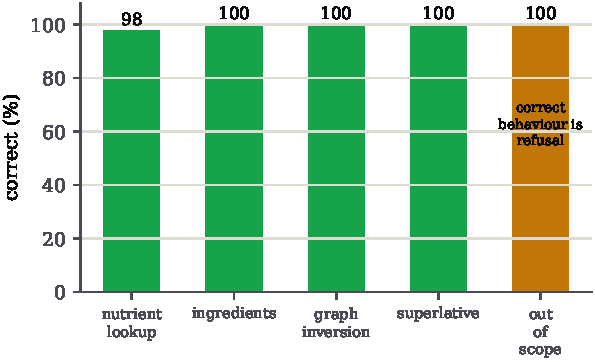
\includegraphics[width=0.72\textwidth]{figures/rag.pdf}
\caption{Answer correctness by question category on the 76-case gold set. For out-of-scope
questions the correct behaviour is refusal, scored separately so that a fluent answer is
counted as the failure it is.}
\label{fig:rag}
\end{figure}

Overall: \num{98.6\%} of in-scope questions answered correctly, \num{100\%} refusal accuracy
with zero false refusals, \num{100\%} of answers grounded, at a total evaluation cost of
\num{\$0.024}. Ground truth is derived from the knowledge base rather than judged by a
model, since a language-model judge would share error modes with the system under test.

Strict recall@1 reads \num{64.6\%} on nutrient lookups. This is a labelling artefact: every
miss returned a \emph{portion} document where a \emph{macros} document was labelled, and all
17 contained the correct figure. An answerability metric, measuring whether the top hit
contains the requested value, reads \num{100\%}.

The grounding gate caught a genuine hallucination on its first live query. Asked for
per-serving sodium, the model produced \num{983.4}\,mg --- arithmetically correct
($447 \times 2.2$) and derivable from a stated multiplier, but present in no document. The
correction was made to the corpus rather than the tolerance: micronutrient documents now
state both bases explicitly, removing the need to derive.

% ── 4 ────────────────────────────────────────────────────────────────
\section{Discussion}

Four of the five negative results share a shape: an added component that should have helped
did not, because the quantity it was meant to improve was already saturated. The fusion head
had nothing to learn because two correlated members need no per-input weighting. DINOv2
added no diversity because self-supervision did not produce independent errors on this
distribution. Fine-tuning added diversity but too little to move a \num{25{,}250}-image
comparison.

The oracle accuracy --- the ceiling if a perfect combiner always selected a correct member
--- is \num{98.43\%}. Only \num{1.57\%} of test images defeat every model, and inspection
suggests a substantial fraction are Food-101 label noise. Ensemble-based approaches on this
dataset are close to exhausted.

\subsection{Limitations}

\begin{itemize}
  \item Attribution localises weakly (\num{0.87}$\times$ chance) for architectural reasons
        described above; the maps indicate a region, not an object.
  \item Sixty of the 101 nutrition profiles are composed from weighted ingredients rather
        than measured directly, and carry correspondingly more uncertainty.
  \item Abstention is a baseline rule, not a trained out-of-distribution detector, which
        would require non-food negatives.
  \item The knowledge base is closed at 101 categories; anything outside is refused rather
        than estimated.
\end{itemize}

% ── 5 ────────────────────────────────────────────────────────────────
\section{Conclusion}

FoodGenome AI classifies at \num{97.16\%} on a sealed Food-101 test split, reports
confidences that match observed accuracy to within \num{0.6} points of calibration error,
supplies prediction sets with a measured \num{99.56\%} coverage guarantee, and answers
grounded nutritional questions while refusing those it cannot support.

The five negative results are the part we would emphasise. Each concerns a component that a
practitioner would reasonably expect to help, each was tested rather than assumed, and each
failed. Reporting them costs a headline number and buys something more useful: a defensible
account of where the remaining headroom is not.

% ── References ───────────────────────────────────────────────────────
\begin{thebibliography}{9}
\small
\bibitem{bossard2014} L.~Bossard, M.~Guillaumin, and L.~Van~Gool.
  Food-101 -- Mining Discriminative Components with Random Forests. \emph{ECCV}, 2014.
\bibitem{zhai2023} X.~Zhai, B.~Mustafa, A.~Kolesnikov, and L.~Beyer.
  Sigmoid Loss for Language Image Pre-Training. \emph{ICCV}, 2023.
\bibitem{fang2023} Y.~Fang et al.
  EVA-02: A Visual Representation for Neon Genesis. \emph{arXiv:2303.11331}, 2023.
\bibitem{oquab2023} M.~Oquab et al.
  DINOv2: Learning Robust Visual Features without Supervision. \emph{TMLR}, 2024.
\bibitem{guo2017} C.~Guo, G.~Pleiss, Y.~Sun, and K.~Q.~Weinberger.
  On Calibration of Modern Neural Networks. \emph{ICML}, 2017.
\bibitem{sadinle2019} M.~Sadinle, J.~Lei, and L.~Wasserman.
  Least Ambiguous Set-Valued Classifiers with Bounded Error Levels. \emph{JASA}, 2019.
\bibitem{angelopoulos2021} A.~N.~Angelopoulos and S.~Bates.
  A Gentle Introduction to Conformal Prediction. \emph{arXiv:2107.07511}, 2021.
\bibitem{cormack2009} G.~V.~Cormack, C.~L.~A.~Clarke, and S.~Buettcher.
  Reciprocal Rank Fusion Outperforms Condorcet and Individual Rank Learning Methods.
  \emph{SIGIR}, 2009.
\bibitem{selvaraju2017} R.~R.~Selvaraju et al.
  Grad-CAM: Visual Explanations from Deep Networks via Gradient-Based Localization.
  \emph{ICCV}, 2017.
\bibitem{darcet2024} T.~Darcet, M.~Oquab, J.~Mairal, and P.~Bojanowski.
  Vision Transformers Need Registers. \emph{ICLR}, 2024.
\bibitem{mcnemar1947} Q.~McNemar.
  Note on the Sampling Error of the Difference Between Correlated Proportions.
  \emph{Psychometrika}, 1947.
\end{thebibliography}

\end{document}
